\documentclass[conference]{IEEEtran}

\usepackage{babel}
\usepackage[table]{xcolor}
\usepackage{collcell}
\usepackage{hhline}
\usepackage{pgf}
\usepackage{multirow}

\def\colorModel{hsb} 

\newcommand\ColCell[1]{
  \pgfmathparse{#1<850?1:0}  %Threshold for changing the font color into the cells
    \ifnum\pgfmathresult=0\relax\color{white}\fi
  \pgfmathsetmacro\compA{0}      %Component R or H
  \pgfmathsetmacro\compB{#1/1500} %Component G or S
  \pgfmathsetmacro\compC{1}      %Component B or B
  \edef\x{\noexpand\centering\noexpand\cellcolor[\colorModel]{\compA,\compB,\compC}}\x #1
  } 
\newcolumntype{E}{>{\collectcell\ColCell}m{0.8cm}<{\endcollectcell}}  %Cell width
\newcommand*\rot{\rotatebox{90}}

\begin{document}

\title{Bayesian networks and other machine learning techniques for sports predicting and betting}

\author{\IEEEauthorblockN{Maj Gaberšček}
\IEEEauthorblockA{Faculty of Computer and Information Science, \\ Večna pot 113, 1000 Ljubljana, Slovenia \\
Email: mg5781@student.uni-lj.si}}


\maketitle

\begin{abstract}
This paper is an attempt to evaluate different machine learning techniques and methods in regard to predicting
sports (football) results. An experiment has been conducted, where we used Bayesian network, Naive Bayes, 
Neural network and $k$-NN in order to predict outcomes of football games as well as possible. An outcome
of a game has been predicted based on form of both opponents (past results of each team). Best model
in this regard is the Naive Bayes, which has managed to achieve accuracy of almost 50\%. Lastly, we have looked
at parameter effect on prediction results, such as data size, $k$ for $k$-NN algorithm and hidden layer size
for Neural Network. The described models are not good enough, to profit in a betting market.

\end{abstract}

\IEEEpeerreviewmaketitle

\section{Introduction}

This paper was written as an attempt to investigate the area of sports predicting.
Sports predicting is mainly used by bookmakers, in order to offer bets, that do 
not produce loss of profit. But on the other hand, odds should be as fair (high) as possible
in order to attract more and more gamblers. So predicting the result of a game as accurately
as possible is the essence of every bookmaker. This article (and experiment) focuses on 
predicting the result of football matches in term of home win (home team scores more goals),
draw (same goal amount for each team) and away win (away team scores more goals).

First chapter of this paper contains information about related work. This includes a 
short recap of discoveries regarding sports results predicting and also a summary of 
new discoveries in regard to betting on sports events.

Second chapter talks about the experiment we have conducted. We describe how we have obtained 
data for our experiment and how the data has been processed in order to be suitable for some 
machine learning techniques. We also report, which machine learning techniques we have used in 
our experiment. Then, we talk about the output data, that the algorithms return and how we 
have compared results with each other. We also discuss, which metrics 
for evaluation are useful, and which among them actually matter the most for our 
experiment (and in general, which metrics matter the most to bookmakers).

Third chapter of this paper focuses on results of our experiment. There, we compare 
different machine learning methods, that have been applied to our data and 
evaluate each one, in regard to metrics. We also discuss, how data size affects the quality 
of our prediction. We compare returned probabilities for different match results, 
to probabilities, that were given by bookmaker. Finally, we decide, whether our models are 
able to beat the odds by chosen bookmaker or not.

Fourth and final chapter is called \emph{Conclusion}, where all important results are
discussed. We will also evaluate our whole experiment and talk about the possible further work 
there.
 
\hfill December 29, 2022

\section{Related Work}

Unsurprisingly, a lot of work has already been done in this area, as sports betting is a field,
where enormous amount of money is being made every day. Firstly, we will talk about 
Bayesian networks, as this model is proved to have success in beating the betting market 
\cite{Constantinou_2012}.

\subsection{Bayesian networks}

Bayesian networks are a type of probabilistic graphical model, that uses Bayesian 
inference for probability computations. Bayesian networks aim to model conditional 
dependence, and therefore causation by representing the model
in a directed graph. Edges in graph correspond to conditional dependency and 
each node corresponds to a different random variable.

Our goal in this article is to predict the correct type of result for a game, similar 
to the work done in article \cite{Razali_2017}. The author of that article used Bayesian
nets on all available statistics of games and achieved 75 percent accuracy. Although it must 
be stated, that the author used match statistics to predict the result of the same match. That is not
particularly useful, as match statistics cannot be known before the game. In this article,
we will try to predict match result, only using data, that was already known \textbf{before}
the game started (so the prediction could be used for betting in real life).

\subsection{Sports predicting}

Betting in sports started with horse racing in the early 1900s \cite{lang2016sports}. Although 
betting was not always legal (depends on a specific country), that did not stop people 
to still gamble on sports events. That's why correctly predicting probabilities of sports 
results has been very important to bookmakers, ever since betting existed. Therefore
machine learning was a very interesting option for bookmakers to consider, as it 
was very objective and it used math and algorithms to predict results. With machine 
learning, bookmakers could also offer odds for games and competitions, that they 
were not so very familiar with.

First attempt to predict sports results with the help of machine learning was in
1977, where the author of article \cite{Stefani_1977} used a technique called 
\textit{least squared model}. That model was used to predict strength of opposing 
teams with goal scoring distribution matrix. Observed accuracy in that model 
was 72 percent for college football games, 68 percent for pro 
football games and 69 percent for college basketball games.

First recorded usage of Bayesian networks in attempt to predict football results was used in
year 2001, in article \cite{Rue_2001}. The authors took an applied statistician's 
approach to the problem, suggesting a Bayesian dynamic generalized linear model to 
estimate the time-dependent skills of all teams in a league and to predict the next 
week-end's football matches.

Paper \cite{Joseph_2006} from 2006 compared expert constructed Bayesian networks' 
ability to predict football results with other machine learning algorithms, such as 
decision tree learner, MC4, Naive Bayes learner, Data driven Bayesian nets (which we 
will be using in our experiment), $K$-nearest neighbours, etc. The results from there 
confirmed, that Bayesian nets have great potential for predicting sport results, as the 
authors had predictive accuracy of almost 60 percent, compared to second best algorithm, 
$K$-nearest neighbours, which had an accuracy of little above 50 percent. Data, that 
the authors  used for prediction, were home advantage, opposition team quality and 
characteristics of team's best players.

In 2010, article \cite{Baio_2010} proposed Bayesian hierarchical model, to predict the number of
goals scored by the two teams in each match.

\subsection{Betting in sports}

This sub chapter contains some information about betting and explains some of the 
technical terms, such as \textit{odds}. So if you are already familiar with betting, 
you are free to skip this part.

Betting on sports events is almost as old as sport events itself. Bookmakers usually 
offer odds on some event. Odds tell bettors how much money they will receive, if that 
event happens. Odds are therefore directly related to the probability of the event. If 
probability of an event is higher, the odds for it will naturally be lower. Bookmakers also
never offer totally fair odds. That way they assure themselves of a guaranteed profit, over 
a long time period. For example, if a probability of an event is expected to be 50 percent,
bookmakers will never offer to pay out double of what you bet, but a little less. For example,
bookmaker \textit{bet365} (British online gambling company, whose odds is used in this
paper), offers to pay out 1.90 times your bet, for an event with probability of 50\%. So the
for this event are $1.90$.

Profiting from a betting market has also been extensively studied in the past. People sometimes
compare odds from different bookmakers, to find an arbitrage strategy. Profiting from an 
inefficient association football gambling market has been studied in article 
\cite{Constantinou_2013} from 2013. In the paper, a Bayesian network is used for forecasting
match outcomes. Profitability, risk and uncertainty are evaluated in there. Although the author
presented a model, that is less complex then some previous ones, it returned better results.
The model considers both objective and subjective information for prediction.  However, it is
important to point out, that the model, which generated profit, was critically dependent on the
knowledge of the expert. Performance, generated only on data, would not be as successful.

\section{Experiment description}

This chapter contains the description of how the experiment was conducted.

\subsection{Tools used}

The data tables were acquired from the web page \emph{Football-Data.co.uk}, and were in the
\texttt{.csv} form. Then data was processed with a programming language \texttt{Python} and 
its library \texttt{pandas}. After that, we applied different machine learning algorithms from
\texttt{scikit-learn} package \cite{scikit-learn}. Bayesian networks were applied 
from the \texttt{pomegranate} library. Returned data was further processed 
with \texttt{pandas} and \texttt{numpy}. All the plots, displayed in this paper, were drawn by the 
\texttt{matplotlib} library.

\subsection{Data}

Data describes every football game of Spanish first division, La Liga (Primera División), 
from season 2013/2014 to 2021/2022. Since each season has 380 games, total data set contained 
3420 games. Every game was a row in the data frame and for each game, the columns represented 
the stats from the game. Some data was unnecessary for match result prediction, for example
number of yellow cards from each game. Important statistics, that was later used in 
model construction, was:
\begin{itemize}
    \item home team name,
    \item away team name,
    \item home team number of scored goals,
    \item away team number of scored goals,
    \item result of the game (home win, away win or draw),
    \item home team number of shots,
    \item away team number of shots,
    \item home team number of corners,
    \item away team number of corners,
    \item bet365 odds for home win,
    \item bet365 odds for away win,
    \item bet365 odds for draw
\end{itemize}

It is important to point out, that data in this form cannot be used to predict results. 
The data was being acquired during the game, but our prediction must be made before the game.
It would of course be pointless to predict the result of the game, if we had already known,
how much goals any of the teams had scored. So we needed to find a way, to predict a result 
of the game, without using that same game's data. We did that by using data from games, that 
happened before the match, that we are predicting. That procedure is described in the next
subsection (\textit{Data processing}).

Odds data will be used to compare our algorithm's predicted probabilities with bookmaker's
predicted probabilities.

\subsection{Data processing}

In order to transform the data, so we could construct models for predicting, we firstly 
dropped those columns, which were not needed for predicting. Then each game was assigned a 
unique index. An iteration through data frame was performed, in order to obtain each team's
order of playing. A new dictionary was defined, where team names were keys and values were
ordered lists of game indexes. 

Then another iteration was made through the original data frame. For each played game, we
looked for 5 previous games for home and away team. The general idea behind this was, 
that we determined strength of a team, based on its previous results. For example,
if a team played well in the past 5 games (it scored many goals, conceded only a few, etc.),
we assume, that it will win with a higher probability, than a team, which did not 
play so well. Basically, we are determining team's strength by its recent form. 

If one team did not have the data of previous 5 games, we left out that match. Usually
that happened with newcomers from the lower division and their first 5 games of the season.

In the end, we got a new data frame, with 3317 games (rows) and the following columns:
\begin{itemize}
    \item \textit{index}: unique index, assigned to each game;
    \item \textit{result}: final result of the game (home win, draw or away win),
    \item \textit{odds\_home}, \textit{odds\_draw} and \textit{odds\_away}: bet365 odds for each possible outcome of the game;
    \item \textit{points\_home} and \textit{points\_away}: points, that home and away team scored in the last 5 games. Note,
    that a team gets 3 points for a win, 1 point for a draw and 0 points for a loss;
    \item \textit{goals\_scored\_home} and \textit{goals\_scored\_away}: a sum of goals, scored in past 5 games for home and away
    team;
    \item \textit{goals\_conceded\_home} and \textit{goals\_conceded\_away}: a sum of goals, conceded in past 5 games for home 
    and away team;
    \item \textit{shots\_given\_home} and \textit{shots\_given\_away}: a sum of shots given, in past 5 games for home 
    and away team;
    \item \textit{shots\_conceded\_home} and \textit{shots\_conceded\_away}: a sum of shots, conceded in past 5 games for home 
    and away team;
    \item \textit{corners\_difference\_home} and \textit{corners\_difference\_away}: a sum of corner differences for home and away team, it the past 5 games. Note, that corner difference is calculated by subtracting opponent's corners from team's corners. 
\end{itemize}

Columns \textit{index} and \textit{odds} are in the data frame just for analysis purposes. 
They were not used in building models. All the other columns contain data, that was already
available, before the game was played (for exception of column \textit{result}). Therefore, 
we can use this data to construct our models for predicting final results of a game.

Note, that time consumption to build Bayesian networks with \texttt{pomegranate} package 
grows exponentially with number of variables. That is why we could not use all the variables 
to build the network in the experiment, so we had to pick the most important ones. As it 
turned out, the most features that could be used was bounded to 7. We decided to use the 
columns that describe final result, points collected, shots given and shots conceded statistics 
for both teams.

Other machine learning algorithms used all the columns (except for odds).

\subsection{Machine learning algorithms used}

The purpose of building our model, was firstly, to predict the game result as well as possible,
but also secondly to see if our prediction can profit in the betting market. For example,
if our algorithm predicts a home win to be the most probable final result and the bookmaker
also offers lowest odds on home win, we could not tell for sure if our prediction would be
sufficient to profit. That is why we need our algorithms to return \textbf{probabilities} for
each game result. That way we can see, which result is profitable to bet on.

For that purpose, we only used \textbf{probabilistic classifiers}: Bayesian network, Naive
Bayes classifier, Neural network (multilayer perceptron) and $k$-nearest neighbours algorithm 
(for $k=5$). All of this methods return probabilities for each class (home win, away win or draw).
% TUKAJ DODAJ ŠE OPISE VSEH MODELOV

\subsection{Metrics for evaluation}

In order to evaluate our predictions for different models, we will use standard metrics for 
evaluating probabilistic classifiers. 

The most important metric will be \textbf{Brier score}, which is defined as 
$$\frac{1}{N} \sum_{i=1}^{N} \sum_{t=1}^{R} {(P(o_{ti}) - o_{ti})^2},$$ in which $R$ is the
number of possible classes of an event and $N$ the overall number of instances (size of our
test data). $P(o_{ti})$ is the predicted probability (returned by our model) of class $t$ 
to occur in instance $i$. $o_{ti}$ is 1 if $i$-th event is of class $t$ and 0 otherwise. 
Better models have smaller 
Brier score.

We will not be calculating the \textbf{log-loss} metric, because our data is far too large 
for personal computer's numerical precision.

From here on, we will assume, that our model predicted the outcome, whose prediction 
percentage will be the highest. 

Second metrics will be \textbf{precision} for each class. Precision refers to the number of 
true positives divided by the total number of positive predictions. The most important will 
be the precision for class \textit{home win}, as this class should have overall the highest 
probability of occurrence. We do not want our model to predict too many home wins.

We will also calculate \textbf{recall} for every class, which is calculated as number of true
positives being divided by total number of positive outcomes. The most important will again be the
recall for class \textit{home win}. For example, a draw is harder to predict and usually most unlikely to happen, 
even if two teams are of a similar strength. That is why we would have a lot of false negatives there.

To merge both precision and recall, we will also calculated the \textbf{F1 score}.

Next metric, that we will be using, is the \textbf{confusion matrix}. While this is not
exactly a metric, it will still provide with rich insight in our model's capability 
to predict a correct most probable result.

Last metric that we will be using will be \textbf{betting profitability}. We will 
compare returned probabilities with betting odds. We will assume to bet if we find a 
profitable combination and not to bet, if we do not. For example, assume that the returned 
probabilities are 50\% for a home win, 30\% for a draw and 20\% for an away win. If bookmaker 
offers equal odds of 2.9 for each outcome, it is most profitable to bet on home win with 
expected profit $$E(profit) = 1.9 \cdot 0.5 - 1 \cdot 0.5 = 0.45, $$
as we profit 1.9 times our stake with probability of 50\% (home win) and lose invested money
with 50\% probability (away win or draw). However, if bookmaker would offer odds of 1.9 for
home win, 3.2 for draw and 4.8 for away win and model would return the same probabilities, no
bet would be expected to return profit. In that case, we decide not to bet any money, so the
betting profitability in that case would be 0. Then we will look at results that happened 
in real life and calculate how much money we would make or lose with our bets on average. That way 
we will calculate our betting profitability for each model. Better models will have bigger profit 
(smaller loss).

\section{Results}

In this chapter, experiment results are described. We evaluated each algorithm
in regard to metrics, that had been described before. The most important aspect of evaluation
will be interpreting the confusion matrix. That way we can get an insight into strengths 
and liabilities of each model.

\subsection{Evaluation}

As an attempt to evaluate our model, we performed a $k$-fold cross validation
for $k=10$. That means that we grouped our data into 10 equally sized groups. We 
chose the first group as our test data and created models from the other 9 
groups. After that, we tested our models on test data (first group). We save the
returned metrics and repeat the procedure, just that this time second group of our data 
will be for testing and models will be build from other nine groups. After repeating this
procedure for each group, we calculate averages of each metric and sum all the elements
of confusion matrix. 

First metric, that is used for evaluation, is the Brier score. 

\begin{table}[!ht]
    \centering
    \begin{tabular}{ll}
        model & Brier score \\ \hline
        \textbf{Neural network} & 206.651 \\ 
        \textbf{Naive Bayes} & 212.93 \\ 
        \textbf{Bayesian network} & 213.165 \\ 
        \textbf{k-NN} & 243.136 \\ 
    \end{tabular}
\end{table}

As stated in chapter \textit{Metrics for evaluation}, better models will have a lower 
Brier score. Neural network has a lowest Brier score, followed by Naive Bayes, which has 
a similar value as Bayesian network. Algorithm $k$-NN has the worst Brier score.

If we compare each model's accuracy, the below table tells us, that Naive Bayes has a 
highest accuracy of almost 50 percent, closely followed by Neural Network.

\begin{table}[!ht]
    \centering
    \begin{tabular}{ll}
        model & accuracy \\ \hline
        \textbf{Naive Bayes} & 0.491 \\ 
        \textbf{Neural network} & 0.482 \\ 
        \textbf{Bayesian network} & 0.469 \\ 
        \textbf{k-NN} & 0.433 \\ 
    \end{tabular}
\end{table}

Next table has data about precision and recall for \textit{home win} class. The F1 score is also
calculated.

\begin{table}[!ht]
    \centering
    \begin{tabular}{llll}
        model & precision & recall & F1 score \\ \hline
        \textbf{Bayesian network} & 0.482 & 0.895 & 0.624 \\ 
        \textbf{Naive Bayes} & 0.565 & 0.695 & 0.622 \\ 
        \textbf{Neural network} & 0.535 & 0.741 & 0.612 \\ 
        \textbf{k-NN} & 0.503 & 0.694 & 0.582 \\ 
    \end{tabular}
\end{table}


If we compare the trade off between precision and recall for each model, Bayesian network
has the highest F1 score. However, as we can see from the table, that the recall is quite high and
precision is low. That means, that the model predicted a lot of false positives and not a lot 
of false negatives. That tells us, that if the outcome was indeed a \textit{home win},
Bayesian network was very successful at predicting, but if the outcome was not a \textit{home
win}, model still falsely predicted that outcome many times. F1 score optimizes combination 
of precision and recall. 

However, in this example, precision and recall are calculated only for \textit{home win}
class. While we can state, that Bayesian network is indeed the best model for predicting 
\textit{home wins}, we cannot imply for sure, that this model is also best for other predictions.
Another example to confirm this will be to define a simple trivial model, that predicts a 
home win in every game, regardless to statistics. That model would have a recall of 1, as it
would never falsely predict an outcome, if that outcome would be a home win. It would have
a precision of 0.45, as 45\% of all games in our data frame resulted in a home win. So the F1
score would be: $$F1 = \frac{2 \cdot precision \cdot recall}{precision + recall} = 0.62,$$
which would still be better than, for example Neural network. So the F1 score is not really
as relevant for our models.

The profit metric will be analyzed in the last subsection of this chapter, \textit{Beating the
bookmakers}. The last and most important aspect of model evaluation is interpreting the 
confusion matrix for each model. 

\begin{figure}[!ht]
\begin{center}
\newcommand\items{3}   %Number of classes
\arrayrulecolor{white} %Table line colors
\noindent\begin{tabular}{cc*{\items}{|E}|}
\multicolumn{1}{c}{} &\multicolumn{1}{c}{} &\multicolumn{\items}{c}{Predicted} \\ \hhline{~*\items{|-}|}
\multicolumn{1}{c}{} & 
\multicolumn{1}{c}{} & 
\multicolumn{1}{c}{\rot{home win}} & 
\multicolumn{1}{c}{\rot{draw}} & 
\multicolumn{1}{c}{\rot{away win}} \\ \hhline{~*\items{|-}|}
\multirow{\items}{*}{\rotatebox{90}{Actual}} 
&home win   & 1359   & 19  & 140   \\ \hhline{~*\items{|-}|}
&draw       & 731   & 11  & 104   \\ \hhline{~*\items{|-}|}
&away win   & 741   & 20   & 183   \\ \hhline{~*\items{|-}|}
\end{tabular}
\end{center}
\caption{Confusion matrix for Bayesian network}
\label{conf_mat_bn}
\end{figure}

First confusion matrix is for Bayesian network, presented in Figure \ref{conf_mat_bn}. 
By observing the matrix, we can clearly see, where the problem of this model is. The model
predicts a match to end in a home win outcome way too often. Even in matches, where the away team
won (which is the opposite of home team winning), the model still mostly predicted home wins. 

Even when the model predicted an away win or a draw, it still did not do well. For example, 
in cases where model supposed an away win, it still did not predict correctly more than half
times (it predicted an away win with precision of 42.8\%). With more than 800 actual matches
ending in a draw, Bayesian network predicted only 50 games to end in a draw. 

It is therefore safe to say, that the Bayesian networks did not meet with the expectations. 
It must however be pointed out, that we used fewer statistics to build this model, due to time
complexity. Therefore we expected for the results to not be as accurate as for other models.

\begin{figure}[!ht]
\begin{center}
\newcommand\items{3}   %Number of classes
\arrayrulecolor{white} %Table line colors
\noindent\begin{tabular}{cc*{\items}{|E}|}
\multicolumn{1}{c}{} &\multicolumn{1}{c}{} &\multicolumn{\items}{c}{Predicted} \\ \hhline{~*\items{|-}|}
\multicolumn{1}{c}{} & 
\multicolumn{1}{c}{} & 
\multicolumn{1}{c}{\rot{home win}} & 
\multicolumn{1}{c}{\rot{draw}} & 
\multicolumn{1}{c}{\rot{away win}} \\ \hhline{~*\items{|-}|}
\multirow{\items}{*}{\rotatebox{90}{Actual}} 
&home win   & 1053   & 266  & 199   \\ \hhline{~*\items{|-}|}
&draw       & 539   & 139  & 168   \\ \hhline{~*\items{|-}|}
&away win   & 504   & 198   & 242   \\ \hhline{~*\items{|-}|}
\end{tabular}
\end{center}
\caption{Confusion matrix for k-NN model}
\label{conf_mat_knn}
\end{figure}

Second confusion matrix is for $k$-nearest neighbours model and can be seen in Figure
\ref{conf_mat_knn}. Similarly as the Bayesian network, $k$-NN predicted
mostly home wins for every actual outcome. So the recall would again be quite low for any other
class than \textit{home win}, although still not as low as for Bayesian network. 

At least the model predicted a more realistic number of draws and away wins. However, 
the precision for both of those classes were not much higher than Bayesian network. This 
model was made for $k=5$. Whether the model could work better for different $k$ is described
in the next subsection, \textit{Parameter effect on results}.

\begin{figure}[!ht]
\begin{center}
\newcommand\items{3}   %Number of classes
\arrayrulecolor{white} %Table line colors
\noindent\begin{tabular}{cc*{\items}{|E}|}
\multicolumn{1}{c}{} &\multicolumn{1}{c}{} &\multicolumn{\items}{c}{Predicted} \\ \hhline{~*\items{|-}|}
\multicolumn{1}{c}{} & 
\multicolumn{1}{c}{} & 
\multicolumn{1}{c}{\rot{home win}} & 
\multicolumn{1}{c}{\rot{draw}} & 
\multicolumn{1}{c}{\rot{away win}} \\ \hhline{~*\items{|-}|}
\multirow{\items}{*}{\rotatebox{90}{Actual}} 
&home win   & 1054   & 124  & 340   \\ \hhline{~*\items{|-}|}
&draw       & 433   & 113  & 300   \\ \hhline{~*\items{|-}|}
&away win   & 381   & 105   & 458   \\ \hhline{~*\items{|-}|}
\end{tabular}
\end{center}
\caption{Confusion matrix for Naive Bayes}
\label{conf_mat_nb}
\end{figure}

Next confusion matrix is presented in Figure \ref{conf_mat_nb}, for the Naive Bayes model. 
Observing the confusion matrix, we can see, that this model predicts far better than the
previous two. For games, where final result was an away win, Naive Bayes predicted an
\textit{away win} (accurately) in most cases. Even when a draw happened, the model did not
predict a \textit{home win} with such big margin to other two predictions, but also predicted
the away team to win quite often. The recall for classes \textit{away win} and \textit{draw} is
considerably higher than those for Bayesian network and $k$-NN.

If we look at precision, it is also quite high (compared to other models), with precision of
33\% for class \textit{draw} and 38\% for \textit{away win}.

\begin{figure}[!ht]
\begin{center}
\newcommand\items{3}   %Number of classes
\arrayrulecolor{white} %Table line colors
\noindent\begin{tabular}{cc*{\items}{|E}|}
\multicolumn{1}{c}{} &\multicolumn{1}{c}{} &\multicolumn{\items}{c}{Predicted} \\ \hhline{~*\items{|-}|}
\multicolumn{1}{c}{} & 
\multicolumn{1}{c}{} & 
\multicolumn{1}{c}{\rot{home win}} & 
\multicolumn{1}{c}{\rot{draw}} & 
\multicolumn{1}{c}{\rot{away win}} \\ \hhline{~*\items{|-}|}
\multirow{\items}{*}{\rotatebox{90}{Actual}} 
&home win   & 1134   & 128  & 256   \\ \hhline{~*\items{|-}|}
&draw       & 515   & 96  & 235   \\ \hhline{~*\items{|-}|}
&away win   & 482   & 97   & 365   \\ \hhline{~*\items{|-}|}
\end{tabular}
\end{center}
\caption{Confusion matrix for Neural network}
\label{conf_mat_nn}
\end{figure}

Last confusion matrix belongs to Neural network model and is show in Figure \ref{conf_mat_nn}.
It seems as Neural network again has the home win bias as in all three actual outcomes, the
model mostly predicted the \textit{home win} class. The recall is again low for \textit{draw}
and \textit{away win}, 12\% and 39\% respectively.

\subsection{Beating the bookmakers}

Here we will compare the algorithms ability to compete with the bookmaker. The below table
gives us average profit per bet of each model. The betting simulation was performed as
described in chapter \textit{Experiment description}, subsection \textit{Metrics for
evaluation}.

\begin{table}[!ht]
    \centering
    \begin{tabular}{|l|l|}
    \hline
        \textbf{model} & average profit per bet \\ \hline
        \textbf{Naive Bayes} & -0.0626 \\ \hline
        \textbf{Bayesian network} & -0.1078 \\ \hline
        \textbf{Neural network} & -0.1142 \\ \hline
        \textbf{k-NN} & -0.1202 \\ \hline
    \end{tabular}
\end{table}

As we can see from the table, no models generated profit. Naive Bayes generated a loss of 6\%
and all other models generated a loss of more than 10\%. That means, if we would bet an euro 
on outcome, proposed by Naive Bayes model, we would lose 6 cents on average. We must of course
remember, that betting odds are not exactly fair. In fact, if betting completely 
randomly and implying, that bookmaker correctly calculated probabilities for each result, 
we would averagely generate a loss of a bit more than 6\%. So, taking that into consideration,
our \textbf{best} model generates a similar loss to a random algorithm. That just proves, that
our models are not good enough to beat the odds or to even predict a better outcome than
bookmakers. That was an expected result.

We will see if by tweaking the parameters of results, we could be able to generate less loss.
That will be described in the next subsection \textit{Parameter effect on results}.

For the conclusion of the betting chapter, we will assume, that odds generated by bookmaker
bet365 resemble true probabilities. We will compare which model returns probabilities most similar to
bookmaker's. We will do that by defining another metric, \textbf{modified Brier score}
$$\frac{1}{N} \sum_{i=1}^{N} \sum_{t=1}^{R} {(P_{model}(o_{ti}) - P_{bet365}(o_{ti}))^2},$$
where $P_{model}(o_{ti})$ is probability of an outcome $o_{ti},$ returned by model and 
$P_{bet365}(o_{ti})$ is bookmaker's probability of the same outcome. We will imply, that 
odds 2 resemble a 50\% probability. Even though that is not completely correct, it will be 
the same for every model, so it does not really matter. The results are visible in the table
below:

\begin{table}[!ht]
    \centering
    \begin{tabular}{|l|l|}
    \hline
        \textbf{model} & modified Brier score \\ \hline
        \textbf{Neural network} & 20.0 \\ \hline
        \textbf{Bayesian network} & 24.1 \\ \hline
        \textbf{Naive Bayes} & 25.2 \\ \hline
        \textbf{k-NN} & 52.7 \\ \hline
    \end{tabular}
\end{table}

From the table we can conclude, that Neural network returns probabilities, that are the 
closest to bookmakers'. $k$-NN's returned probabilities are by far the worst.

\subsection{Parameter effect on results}

In this subsection, we are going to explore how the changing of parameters affect final 
results and model evaluation. 

Firstly, we will look at how changing the $k$ parameter in $k$-NN affect our prediction.
We again performed a 10-fold cross validation for different $k$ in range from 5 to 30.

First plot (Figure \ref{profit-knn}) shows average profit in relation to $k$. We can see, 
that the profit was maximized for $k$ around 70. That means that our model should find 70 
other matches, with data that is most similar to the game, and predict in regard to that.

\begin{figure}[!ht]
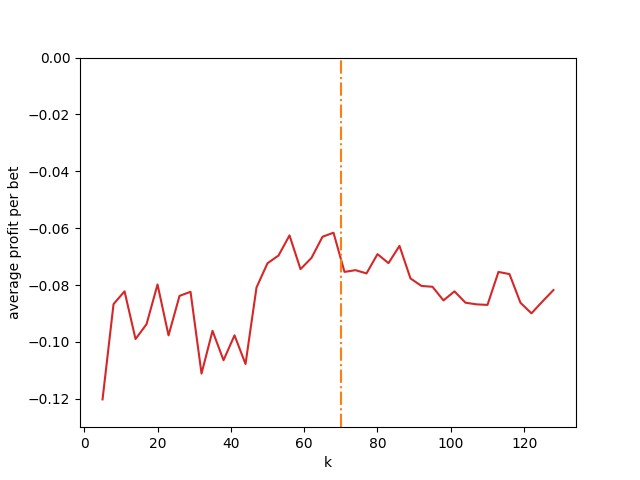
\includegraphics[width=0.5\textwidth]{profit_k_knn.png}
\caption{Profit in relation to $k$ for $k$-nearest neighbours model.}
\label{profit-knn}
\end{figure}

\begin{figure}[!ht]
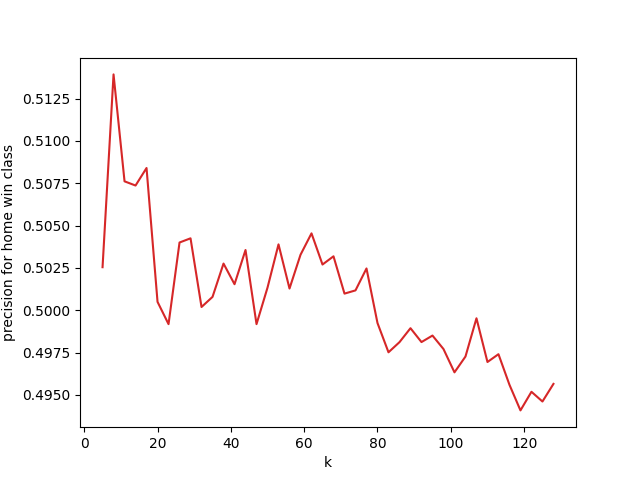
\includegraphics[width=0.5\textwidth]{precision_k_knn.png}
\caption{Precision in relation to $k$ for $k$-nearest neighbours model.}
\label{prec-knn}
\end{figure}

The $k$-NN model for $k=5$ had a problem in predicting too many home wins (as discussed 
previously). That resulted in precision particularly low. So we shall compare how precision
grows (or falls) with $k$. The results are presented in Figure \ref{prec-knn}. It seems as if
precision decreases if we are increasing $k$. So manipulating parameter $k$ does not help with
our issue from before, when model predicted too many home wins.

Let's also check, for which $k$ the returned predictions are the closest to bookmaker's 
predicted probabilities. The plot for modified Brier score in relation to $k$ is presented in Figure \ref{mbs-knn}. It looks as if the bigger the $k$, the more similar our predictions are to bookmakers'.

\begin{figure}[!ht]
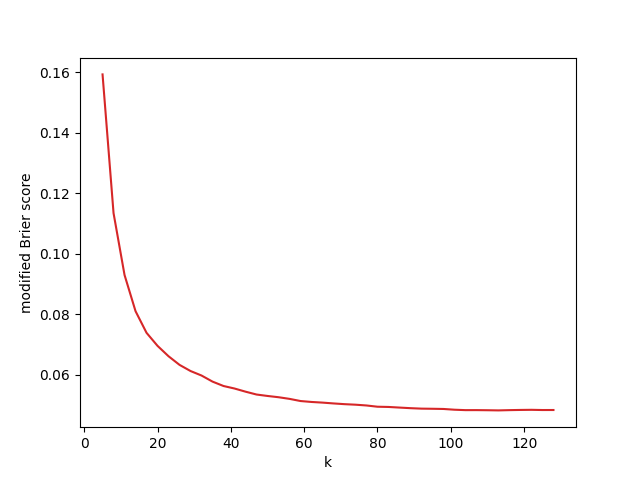
\includegraphics[width=0.5\textwidth]{mbs_k_knn.png}
\caption{Modified Brier score in relation to $k$ for $k$-nearest neighbours model.}
\label{mbs-knn}
\end{figure}

Secondly, we will look at how changing size of our Neural network affects predictions.
We will be changing hidden layer sizes and see how results change. Default model had one
hidden layer with 100 neurons.

It is interesting, that with adding more hidden layers, almost all metrics start getting worse.
If we, for example, visualise our modified Brier score in relation to number of hidden layers 
(Figure \ref{mbs-mlp}), we can see that the more layers we include, the less similar
returned probabilities are to bet365's.

\begin{figure}[!ht]
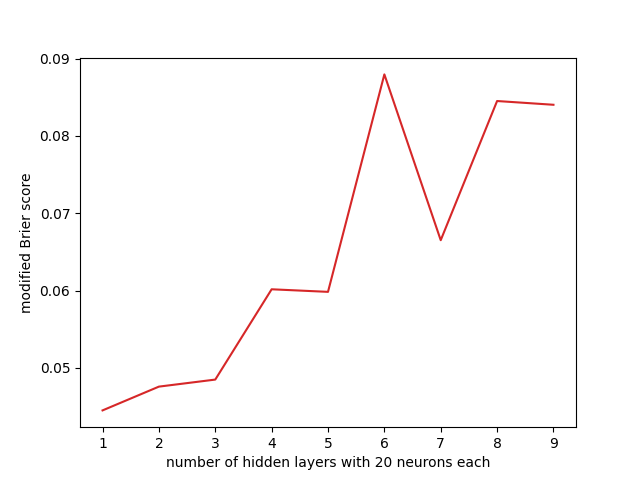
\includegraphics[width=0.5\textwidth]{mbs_layers_mlp.png}
\caption{Modified Brier score in relation to number of hidden layers with 20 neurons.}
\label{mbs-mlp}
\end{figure}

Similar thing happens, if we only include one hidden layer and start increasing number
of neurons. Predictions start getting worse and worse.

Lastly, we will look at how learning data size affects our prediction. We will be using the 
Naive Bayes model and slowly increase learning data size. This time, we will not be using 
the $k$-fold cross validation for testing, but we will pick a fixed size test data of 500
instances.

First plot, Figure \ref{data_size_profit} shows, rise of the profit, if we increase the data
size. However, with limited data, we could never know if Naive Bayes could beat the bookmaker.

\begin{figure}[!ht]
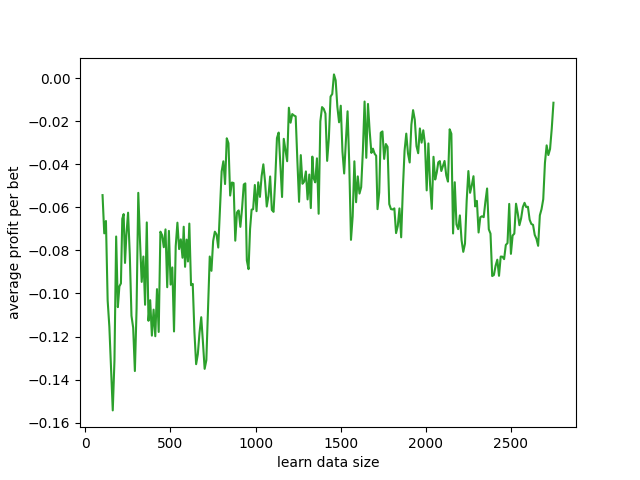
\includegraphics[width=0.5\textwidth]{profit-data_size.png}
\caption{Profit in relation to the size of the learn data frame}
\label{data_size_profit}
\end{figure}

Figure \ref{data_size_brier}, portrays how Brier score decreases with bigger data size. It
can be observed, that the decrease rate settles at data size approximately 1500. That tells us,
that even by adding many more data, we would still not get predictions, that are far more similar,
than bookmaker's. (at least not with Naive Bayes model).

\begin{figure}[!ht]
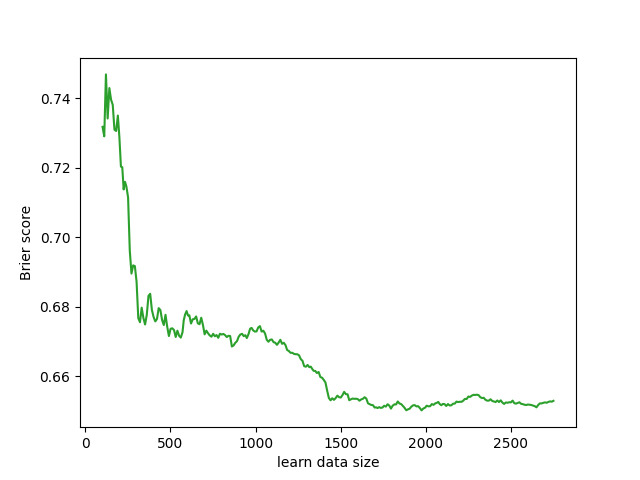
\includegraphics[width=0.5\textwidth]{brier-data_size.png}
\caption{Profit in relation to the size of the learn data frame}
\label{data_size_brier}
\end{figure}

\section{Conclusion}

\section*{Acknowledgment}

\bibliographystyle{IEEEtran}
\bibliography{bibliography} 

\end{document}


